%!TEX root = ../Polito PhD thesis template.tex
% ******************************* Chapter 4 ************************************
% From: Neural Network-Assisted Genetic Optimization of the Multi-Group
%       Energy Structure for Lead-Cooled Fast Reactors
% Source: materials/enanching_multigroup_LFR/lfr_energy_grid/paper/paper.tex
%         tables/ and figures alongside; workflow_LFR.ipynb reproduces numbers
% Bibliography for this chapter: Chapter4/refs_eg.bib (to be added to the
% \bibliography list of the main file; References/references.bib not modified).
% NOTE: the flowchart figure (TikZ) requires in the thesis preamble:
%   \usepackage{tikz}
%   \usetikzlibrary{shapes.geometric,arrows.meta,positioning,fit,backgrounds,calc}
% (tikz also loads xcolor, needed by the \providecolor definitions below).

% Colours defined in the paper preamble and used by the TikZ flowchart
% (\providecolor instead of \definecolor to avoid collisions with other chapters)
\providecolor{serpent}{HTML}{4CAF7D}
\providecolor{fren}{HTML}{E8703A}
\providecolor{nnc}{HTML}{3B7A99}
\providecolor{ga}{HTML}{F2C14E}
\providecolor{newc}{HTML}{1F6FB2}

\chapter{Neural Network-Assisted Optimization of the LFR Multi-Group Energy Grid Driven by Genetic Algorithms}\label{ch:energy-grid}  %CV: ho cambiato il titolo qua

\section{Introduction}

Full-core deterministic simulations of fast reactors, and in particular the
transient analyses for which they are ultimately intended, are performed on a
condensed energy mesh. The number of groups and the placement of their
boundaries determine how faithfully the condensed calculation reproduces a
Monte Carlo reference, and the dependence is neither smooth nor intuitive, since
two structures with the same number of groups can differ by orders of magnitude
in accuracy. The impact of energy collapsing on the integral parameters of a
fast system has been analysed in detail for the neutron
lifetime~\cite{collapsing}, and the identification of the structure itself has
been addressed with several metaheuristics: particle swarm optimization for
thermal lattices~\cite{psoThermal}, genetic algorithms for multigroup searches
in SIMMER~\cite{massoneGA,simmerGA} and for the ARC fusion
reactor~\cite{arcGA}, simulated annealing for sodium-cooled fast
reactors~\cite{sfrSA}, hierarchical division~\cite{hierDiv}, and dedicated
studies for specific systems~\cite{scwr}.

For the lead-cooled fast reactor the problem has been developed along a
consistent line of work~\cite{lfrGA2022,lfrGA2024,prevGA}, culminating in the
multi-configuration formulation of \citet{prevMulti}, in which a single
energy structure is optimized simultaneously for three control-rod
configurations, so that the same grid remains adequate as the core evolves
during a transient. That study reported an observation which motivates the
present one. The genetic algorithm was run from three different random seeds,
referred to as tribes, and the three tribes converged to three different
structures sharing many boundaries but not all of them. Since the tribes differ
only in the initial population, the outcome indicates that the objective
possesses several distinct optima of comparable quality, and that a single run
samples one of them without any indication of which.

The behaviour has a natural explanation in the nature of the problem. The
decision variable is a subset of the internal boundaries of a fine mesh, so that
the search space is combinatorial rather than continuous and contains
$2^{29}\approx5.4\times10^{8}$ elements, on which no notion of gradient exists.
The objective is the product of fifteen terms, each measuring the agreement of a
different physical quantity in a different core configuration, and the terms do
not respond in the same way to the displacement of a boundary: a change that
improves the multiplication factor may worsen the flux distribution. How abrupt
the resulting surface is can be measured on the available data. Among the
structures computed in this work, those differing by exactly one boundary have
joint fitness values that differ by a median of $0.41$ decades in the region of
the best solutions, so that a single bit of the
representation can move the objective by a factor of two and a half. A surface
of this kind possesses many local optima separated by barriers that a
population-based search crosses or does not cross depending on where it starts,
which is precisely what three tribes with three different outcomes indicate.

Two consequences follow. The first is that the result of a single optimization
should not be interpreted as the optimal structure, but as one member of a set
whose extent is unknown. The second is that any statement of general validity
about where the boundaries of a good structure should lie requires many
independent searches, not one. Both consequences call for the same remedy, a higher
number of simulated tribes could provide a better answer to the need to find an optimized
energy grid.

That remedy is not affordable within the workflow shown in \citet{prevMulti}. The fitness of a
candidate structure can only be established by running the reference
calculation, and a population-based search requires one such evaluation for
every individual of every generation. In the present case a single evaluation,
covering the three control-rod configurations, costs on average $46$~s on three cores with
the neutronics module of FRENETIC~\cite{frenetic,freneticBench}, so that one
search of a hundred individuals over a hundred generations amounts to
approximately $383$ core-hours. One thousand such searches would exceed
$380\,000$ core-hours, which places the analysis out of reach.

The present work removes this bottleneck by replacing the evaluation inside the
search with a neural network of the fitness functions, while leaving the
reference solver in charge of the conclusions. The metamodel is used to explore,
to rank, and to propose; every structure that the searches produce is then
recomputed with FRENETIC, and all the quantities discussed in the following
sections are those returned by the solver. The metamodel is therefore an
accelerator of the search and not a substitute for the physics, an arrangement
which also protects the results from the regions in which its accuracy is hard to
learn for the metamodel.

The chapter first defines the optimization problem, reporting in full the
chromosome representation and the fitness functions inherited from
\citet{prevMulti}. It then describes the metamodel, its training and its
accuracy, and identifies the regime in which it is least reliable, since that
regime dictates the role it is given. The resulting workflow, summarized in Figure~\tref{eg:fig:flow}, is presented next,
followed by the analysis of the thousand searches, of the structures they
produce, and of the features those structures have in common.

\begin{figure}[htbp]
  \centering
  \resizebox{\textwidth}{!}{% Flowchart del workflow. Riprende la struttura di quello del lavoro di
% riferimento (Costantino et al.) per renderne immediato il confronto.
% Convenzione grafica: cornice e frecce BLU = introdotto in questo lavoro;
% cornice sottile grigia = ereditato dal workflow di riferimento;
% blocco tratteggiato sbiadito = ciò che il metamodello ha sostituito.
\begin{tikzpicture}[
  font=\footnotesize,
  node distance = 4.2mm and 7mm,
  base/.style    = {rectangle, rounded corners=1pt, align=center, inner sep=3pt,
                    minimum height=7.5mm, text width=32mm},
  old/.style     = {base, draw=black!55, line width=.4pt},
  new/.style     = {base, draw=newc, line width=1.1pt},
  round/.style   = {rounded corners=3.2mm, fill=ga!55},
  serp/.style    = {old, fill=serpent!55},
  frenN/.style   = {new, fill=fren!45},
  netN/.style    = {new, fill=nnc!40},
  greyO/.style   = {old, fill=black!8},
  greyN/.style   = {new, fill=black!8},
  faded/.style   = {base, fill=black!4, draw=black!25, dashed, text=black!40,
                    text width=27mm, minimum height=6mm},
  dec/.style     = {diamond, aspect=1.9, draw=black!55, fill=ga!45, align=center,
                    inner sep=0pt, text width=24mm, font=\scriptsize},
  arO/.style     = {-{Latex[length=1.6mm]}, draw=black!65, line width=.45pt},
  arN/.style     = {-{Latex[length=1.6mm]}, draw=newc, line width=.9pt},
  lbl/.style     = {font=\scriptsize, inner sep=1.5pt},
]

% ── colonna sinistra: riferimento Monte Carlo (invariata) ────────────────
\node[greyO] (fine) {fine-group homogenised\\constants (30 groups)};
\node[serp, below=of fine] (serpent) {Serpent 2\\Monte Carlo};
\node[greyO, below=of serpent] (ref) {reference output\\$k_\mathrm{eff}$, $P$, $\Phi$,
  $\ell_\mathrm{eff}$, $\beta_\mathrm{eff}$};

% ── addestramento del metamodello (nuovo) ───────────────────────────────
\node[frenN, below=8mm of ref] (train) {FRENETIC (NE module)\\$91\,723$ full-core\\evaluations};
\node[netN, below=of train] (nn) {\textbf{neural metamodel}\\hierarchical ensemble};

\draw[arO] (fine) -- (serpent);
\draw[arO] (serpent) -- (ref);
\draw[arN] (ref) -- (train);
\draw[arN] (train) -- node[lbl, right] {training} (nn);

% ── ciclo genetico ──────────────────────────────────────────────────────
\node[old, round, right=30mm of fine] (gen) {generate $N$ individuals};
\node[netN, below=of gen] (eval) {\textbf{evaluate the whole\\population at once}};
\node[old, round, below=of eval] (ff) {joint FF with\\running scaling};
\node[old, round, below=of ff] (sel) {selection};
\node[old, round, below=of sel] (cross) {crossover};
\node[old, round, below=of cross] (mut) {mutation};
\node[dec, below=5mm of mut] (term) {termination\\satisfied?};

\draw[arN] (gen) -- (eval);
\draw[arN] (eval) -- (ff);
\draw[arO] (ff) -- (sel);
\draw[arO] (sel) -- (cross);
\draw[arO] (cross) -- (mut);
\draw[arO] (mut) -- (term);
\draw[arN] (nn.east) -- ++(6mm,0) |- (eval.west);
\draw[arO] (ref.east) -- ++(3mm,0) |- (ff.west);
\draw[arO] (term.east) -- ++(7mm,0) node[lbl, above right, xshift=-6mm] {no}
          |- ([yshift=2mm]eval.east) -- (eval.east);

% ── ciò che il metamodello ha sostituito ────────────────────────────────
\node[faded, right=30mm of eval, yshift=6.5mm] (old1) {C++/Python coupling};
\node[faded, below=2.5mm of old1] (old2) {input generation};
\node[faded, below=2.5mm of old2] (old3) {one solver call\\per individual};
\node[draw=black!25, dashed, rounded corners=1.5pt, inner sep=2.5mm,
      fit=(old1)(old3)] (deadbox) {};
\node[lbl, above=1.2mm of deadbox, text=black!45, align=center, text width=34mm]
     {replaced by the metamodel};
\draw[dashed, draw=black!35, line width=.5pt] (eval.east) -- (deadbox.west);

% ── multi-start e giudizio finale (nuovi) ───────────────────────────────
\node[old, round, below=6mm of term] (tribe) {tribe completed};
\node[new, round, fill=ga!55, below=of tribe] (many) {$1000$ independent\\tribes};
\node[new, round, fill=ga!55, below=of many] (scale) {outcomes on one\\common scale};
\node[new, round, fill=ga!55, below=of scale] (rank) {distinct candidates,\\ranked by fitness};
\node[frenN, below=of rank] (verify) {\textbf{FRENETIC (NE module)}\\verification of the\\best candidates};
\node[greyN, below=of verify] (out) {final ranking\\optimized structure};

\draw[arO] (term) -- node[lbl, right] {yes} (tribe);
\draw[arN] (tribe) -- (many);
\draw[arN] (many) -- (scale);
\draw[arN] (scale) -- (rank);
\draw[arN] (rank) -- (verify);
\draw[arN] (verify) -- (out);
\draw[arN] (many.west) -- ++(-7mm,0) |- node[lbl, left, pos=.25] {new seed} (gen.west);

% ── legenda ─────────────────────────────────────────────────────────────
\node[new, fill=white, below left=14mm and -32mm of out, text width=3mm,
      minimum height=3mm, inner sep=0pt] (lg1) {};
\node[lbl, right=1.5mm of lg1, anchor=west] {introduced in this work};
\node[old, fill=white, below=2.5mm of lg1, text width=3mm,
      minimum height=3mm, inner sep=0pt] (lg2) {};
\node[lbl, right=1.5mm of lg2, anchor=west] {inherited from the reference workflow};
\node[faded, below=2.5mm of lg2, text width=3mm, minimum height=3mm, inner sep=0pt] (lg3) {};
\node[lbl, right=1.5mm of lg3, anchor=west, text=black!45]
     {no longer required};

\begin{scope}[on background layer]
  \node[fill=ga!12, rounded corners=2mm, fit=(gen)(term)(mut), inner sep=3.5mm] {};
\end{scope}
\end{tikzpicture}}
  \caption[Workflow adopted in this work]{Workflow adopted in this work, drawn for direct comparison with the
  one of \citet{prevMulti}. Boxes and arrows outlined in blue are introduced
  here, those with a thin grey outline are inherited unchanged, and the faded box
  on the right is the per-individual call to the solver that the metamodel
  replaces. The shaded area encloses the genetic loop.}
  \label{eg:fig:flow}
\end{figure}


\section{Definition of the Optimization Problem}

\subsection{Reference Data and Fitness Functions}

Serpent~2 is used to generate, for each core configuration, both the reference
values of the integral parameters and the spatially homogenised fine-group
constants, evaluated at isothermal conditions with fuel and coolant at $673$~K.
The data are collapsed onto a fine structure of 30 groups whose boundaries are
extracted from the ECCO-33 grid, chosen so that few groups describe the thermal
and the fast regions where the Monte Carlo statistics are poorest. That
30-group structure constitutes the pool of boundaries available to the
optimization, and the case study is the ALFRED core, in the specification of
the lead-cooled fast reactor benchmark coordinated by the Nuclear Energy
Agency~\cite{neaBench}.

Three control-rod configurations are considered simultaneously, shown in
Fig.~\tref{eg:fig:core} together with the radial layout of the core: rods fully
withdrawn, with the absorber entirely below the active fuel; rods partially
inserted, with the absorber facing the fuel over a length of $28$~cm; and rods
fully inserted, with the absorber covering the whole active height. The multiplication factor of the reference calculation falls from $1.096$ to
$1.072$ and then to $1.019$ across the three, and the three are denoted in
what follows by the subscripts $\mathrm{out}$, $\mathrm{partial}$
and $\mathrm{in}$ respectively. For a candidate structure $I$, the agreement with
the Monte Carlo reference is measured by five fitness functions per
configuration~\cite{prevMulti}. Three of them concern integral quantities,
%
\begin{equation}
  f_k^I = \left|k^I - k^\mathrm{MC}\right|\times10^5, \qquad
  f_{\beta}^I = \left|\beta_\mathrm{eff}^I - \beta_\mathrm{eff}^\mathrm{MC}\right|
  \times10^5, \qquad
  f_{\ell}^I = \left|\frac{\ell_\mathrm{eff}^I -
  \ell_\mathrm{eff}^\mathrm{MC}}{\ell_\mathrm{eff}^\mathrm{MC}}\right|\times10^2,
  \label{eg:eqn:integral}
\end{equation}
%
namely the multiplication factor, the effective delayed neutron fraction and
the effective neutron lifetime, the last being the adjoint-weighted lifetime
that the reference calculation tallies, and not the generation time, which
differs from it by the multiplication factor. The remaining two concern the
distributions over the $J$ core assemblies,
%
\begin{equation}
  f_P^I = \sqrt{\sum_{j=1}^{J}\left(\frac{P_j^I-P_j^\mathrm{MC}}
  {P_j^\mathrm{MC}}\right)^{2}}, \qquad
  f_{\Phi}^I = \sqrt{\sum_{g=1}^{G}\sum_{j=1}^{J} w_{g,j}
  \left(\frac{\Phi_{g,j}^I-\Phi_{g,j}^\mathrm{MC}}
  {\Phi_{g,j}^\mathrm{MC}}\right)^{2}},
  \label{eg:eqn:distributed}
\end{equation}
%
the flux being weighted by the total importance $\phi\phi^{\ddagger}/v$, the
product of the flux and of the adjoint flux divided by the neutron speed of the
group as tabulated in the reference library, which measures how much the
neutrons of a group contribute to the chain reaction and is examined in
Sec.~\ref{eg:sec:recurring}. All
five are deviations from the reference, so that smaller values indicate a better
structure.

Since the five quantities differ by orders of magnitude and in range of
variability, each is mapped onto the interval $[1,100]$ by the linear scaling
%
\begin{equation}
  h_L : f \longrightarrow 1 + 99\,
  \frac{f-\min_{\forall I\in E}\left(f^I\right)}
       {\max_{\forall I\in E}\left(f^I\right)-\min_{\forall I\in E}\left(f^I\right)},
  \label{eg:eqn:scaling}
\end{equation}
%
where $E$ denotes the set of solutions evaluated so far, and the joint fitness
of a candidate is the product of the fifteen scaled terms, five for each of the
three configurations,
%
\begin{equation}
  FF^I = \prod_{c\in\{\mathrm{out},\,\mathrm{partial},\,\mathrm{in}\}}
  h_L\!\left(f_{k,c}^I\right) h_L\!\left(f_{P,c}^I\right)
  h_L\!\left(f_{\Phi,c}^I\right) h_L\!\left(f_{\ell,c}^I\right)
  h_L\!\left(f_{\beta,c}^I\right).
  \label{eg:eqn:joint}
\end{equation}
%
Before the scaling, the three integral fitness functions are clipped from below
and the flux fitness function is replaced by its base-ten logarithm floored at
unity. The threshold of the clipping is ten pcm, and since
Eq.~(\ref{eg:eqn:integral}) does not express the three functions in the same
units it takes a different numerical value in each. For $f_k$ and $f_{\beta}$,
defined as absolute deviations multiplied by $10^{5}$, ten pcm is the value
ten; for $f_{\ell}$, defined as a relative deviation multiplied by $10^{2}$,
the same ten pcm is the value $0.01$. In all three cases the threshold is a few
times the statistical uncertainty of the reference, which stays below two pcm
on the multiplication factor, below one pcm on the delayed neutron fraction and
at about five hundredths of a per cent on the lifetime. Its purpose is to mark
the level below which a difference between two structures is not treated as an
improvement: a quantity reproduced to within the threshold is clipped and stops
contributing to the ranking, so that the search is directed towards what is
still worth improving, and a term already at the precision of the reference
cannot dominate the product. The logarithmic floor on the flux acts instead as a
compression of scale. All of them are applied identically to the reference
values and to the candidate ones.

\begin{figure}[htbp]
  \centering
  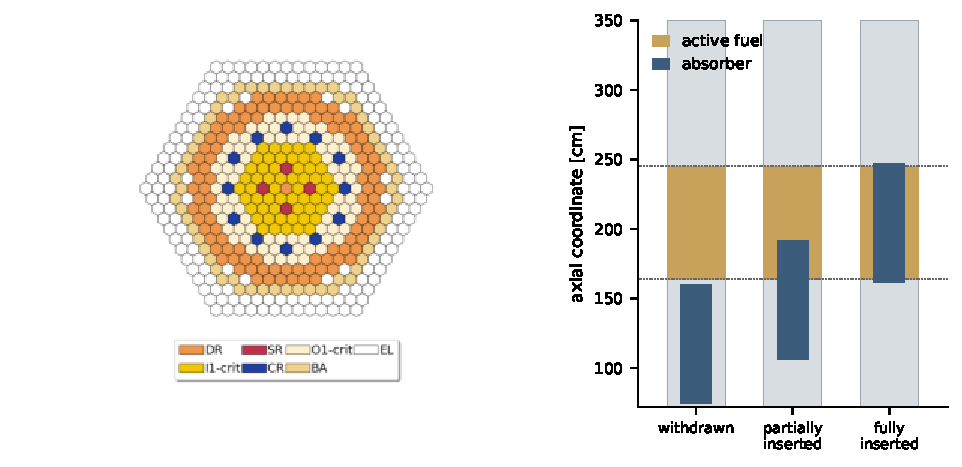
\includegraphics[width=\textwidth]{Chapter4/Figs/fig_core.pdf}
  \caption[The ALFRED core of the NEA lead-cooled fast reactor benchmark]{The ALFRED core, as specified in the NEA lead-cooled fast reactor benchmark. Left, radial
  layout at mid-height: inner and outer fuel assemblies (I1-crit, O1-crit),
  control rods (CR), safety rods (SR), dummy elements (DR), the barrel (BA) and
  the surrounding lead reflector (EL). Right, axial position of the absorbing
  region of a control rod in the three configurations, with the active fuel
  shaded and its extremes marked by the dotted lines. The layout is the one used
  for the FRENETIC calculations and is drawn from the same input.}
  \label{eg:fig:core}
\end{figure}

\subsection{Chromosome Representation}

The optimization variable is the set of internal boundaries retained from the
fine structure. Of the 31 boundaries of the 30-group mesh the two extremes are
fixed, so that a candidate structure corresponds to a subset of the remaining
$H-1=29$ internal boundaries and the design space contains
$2^{29}\approx5.4\times10^{8}$ elements.

The earlier formulations of this problem fixed the number of groups before the
search and left the genetic algorithm to place the boundaries alone, with one
binary gene per internal boundary of the fine mesh stating whether it is
retained. Prescribing $G$ restricts the space that can be reached and excludes
the structures that a different number of groups would make available. Several
chromosome definitions were therefore compared in the line of work that precedes
this one, and the one retained combines the features of the others and carries
the number of groups as a gene of its own, so that $G$ is searched over rather
than imposed~\cite{prevGA}.

The representation adopted here is that polyploid encoding, in the form used in
the multi-configuration formulation of \citet{prevMulti}, reproduced in full because it determines both the
behaviour of the genetic operators and the input of the metamodel. A chromosome
consists of two sets. The first, $\gamma_0$, is a single gene holding the number
of groups $G$ of the structure, constrained to $4\le G\le20$. The second,
$\gamma_1$, is polyploid and contains $P=4$ arrays of $H-1=29$ genes each, one
gene per internal boundary, whose alleles take integer values in $\{0,1,2\}$. An
individual is therefore described by $1+P(H-1)=117$ variables.

Decoding proceeds in two steps. For each internal boundary $i$ the $P$ arrays
are summed into a score
%
\begin{equation}
  s_i = \sum_{p=1}^{P} \gamma_{1,p,i}, \qquad i = 1,\dots,H-1,
  \label{eg:eqn:score}
\end{equation}
%
and the $G-1$ boundaries with the highest score are retained, ties being
resolved by increasing energy index. The polyploid structure gives each boundary
a graded rather than binary expression, so that a boundary can be strengthened
or weakened by mutation without being switched on or off abruptly, which
smooths the effect of the genetic operators on the decoded structure. A repair
operator enforces the bounds on $G$ and the validity of the alleles after
crossover and mutation.


\section{The Metamodel}

\subsection{Training Set}

The metamodel is trained on 91\,723 distinct structures for which the
neutronics module of FRENETIC has been run over the three configurations. The
set was assembled incrementally, over seventeen batches. The first was drawn at
random from the design space; each of the following ones was selected, among the
structures not yet simulated, by the disagreement among the members of an
ensemble of networks -- the variance of their predicted means, in the space in
which the networks are trained -- averaged over the nine quantities that the
model predicts least accurately, namely the multiplication factor, the flux and the generation
time for the three configurations. The criterion was applied with the ensemble
available at the time of each batch, so the acquisition history is not
homogeneous, and the retrospective experiment described below replays it under a
single protocol in order to measure what the accumulated data are worth. A
further 1\,700 structures form an external validation set which is never used
in training nor for early stopping. It did guide the development: the
architectures and trunk widths explored in the preliminary phase were compared
on its coefficient of determination, overall and output by output. The accuracy
figures quoted in this work, which all refer to this set, are therefore not
fully immune from selection effects, and the protection against over-reliance
on them is structural rather than statistical: the workflow described later
verifies with the reference solver every result it uses. The ablation and
reproducibility measurements of the next subsection are evaluated on the same
set, after the architecture had been fixed.

\subsection{Architecture}

The fifteen fitness functions are not independent, since they group into five
physical families, each evaluated for the same three core states. The network
reproduces that organisation. A shared trunk of three fully connected layers of
$1024$, $512$ and $256$ neurons receives the 29-bit description of the structure
together with the number of groups. The trunk feeds five family-level branches
of $128$ and $64$ neurons, each of which feeds three configuration-level
branches of $32$ neurons terminating in the corresponding output. Every hidden
layer uses the ReLU activation, and each configuration branch in fact ends in
two numbers, the predicted value and the logarithm of a variance, whose only
role is in the loss function described below. Parameters are
thus shared to the extent that the physics shares them and specialised where it
does not.

The capacity is the outcome of exploration, not of a rule. The first
configuration adopted was considerably smaller and saturated during the
active-learning campaign, its accuracy no longer improving as data kept
arriving. Since generating the training data was by far the expensive side of
the exercise, the network was the economical one to act on, and architectures,
trunk widths and training parameters were explored extensively to extract more
accuracy from the same data; the sizes above are what that exploration
settled on. The retrospective learning curve reported below confirms that,
after the enlargement, the limit moved back to the data.

An ablation quantifies what each level of the hierarchy is worth, and the result
is not symmetric. Table~\tref{eg:tab:ablation} reports three architectures trained
on the same data with the same reduced protocol, a single network at constant
learning rate. Introducing the five family necks raises the mean coefficient of
determination from $0.9848$ to $0.9908$ and lowers the median relative error
from $1.75$ to $1.50\%$, at the price of a $29\%$ increase in the number of
parameters. Adding the configuration branch below them changes neither figure
appreciably, $0.9905$ and $1.49\%$.

The second comparison rests on differences of four ten-thousandths in the
coefficient of determination and of seven thousandths of a point in relative
error, and margins of that size mean nothing unless the reproducibility of the
training is known. It was therefore measured: five networks of identical
architecture, trained with the identical protocol and differing only in the
random initialisation of their weights, span a range of $0.0031$ in the
coefficient of determination and of $0.24$ points in relative error, with
standard deviations of $0.0013$ and $0.11$. The difference between the two
architectures is thus four times smaller than the scatter between two runs of
the same one, and fifteen times smaller on the relative error. The comparison of
the fifteen outputs one by one leads to the same conclusion: the family necks
improve twelve outputs out of fifteen with respect to the flat network, a
consistent effect, while the configuration branch improves eight out of fifteen,
a proportion indistinguishable from the one expected
if the two architectures were equivalent.

The physical quantity, and not the core configuration, is therefore the
dimension along which the fifteen outputs need separate parameters, and this is
consistent with three configurations that differ only in the position of the
control rods and share the same materials, the same geometry and the same fine
mesh. The production model retains the configuration branch, which was already
present when the ablation was performed and costs $3\%$ additional parameters,
and the measurement gives no reason to retrain without it; it does, however,
identify the family level as the one that carries the architectural gain.

\begin{table}[htbp]
\centering
\caption[Contribution of each level of the hierarchy]{Contribution of each level of the hierarchy, measured on the same
91\,723 configurations and with the same reduced protocol: one network per
architecture, constant learning rate and early stopping. The absolute values are
therefore higher than those of the final ensemble, and only their differences
are meaningful. The last line gives the scatter observed over five networks of
identical architecture differing only in their random initialisation, which sets
the scale below which a difference cannot be read.}
\label{eg:tab:ablation}
\begin{tabular}{@{}p{62mm}ccc@{}}
\toprule
Architecture & Parameters & $R^2$ & Rel.\ err.\ [\%] \\ \midrule
    Shared trunk, fifteen linear heads & 0.70M & 0.9848 & 1.750 \\
    Shared trunk, one neck per family & 0.90M & 0.9908 & 1.501 \\
    Shared trunk, family neck, configuration branch & 0.93M & 0.9905 & 1.494 \\
\midrule
    \emph{Spread over five random initialisations} & & $\pm$0.0013 & $\pm$0.11 \\ \bottomrule
\end{tabular}
\end{table}
Twelve of the fifteen outputs span several orders of magnitude and are learned 
as $\log_{10}(y+10^{-6})$, while the three power fitness functions are learned
directly. Predictions are averaged over an ensemble of five networks trained
from different random initialisations~\cite{deepEnsembles}; the average is taken
in the standardised space in which the networks are trained, which for the
twelve logarithmic outputs amounts to a geometric mean in physical units. The
disagreement among the members of the ensemble also provides the criterion used
to select the configurations added to the training set.

\subsection{Training and Accuracy}

The inputs -- the 29-bit description of the structure and the number of
groups -- and the fifteen targets, in the logarithmic space defined above, are
standardised to zero mean and unit variance, with the scalers fitted on the
training portion alone. An internal validation split, $15\%$ of the $91\,723$
configurations drawn once with a fixed seed, serves for early stopping; it is
distinct from the external validation set, which no training signal touches.

The loss is the Gaussian negative log-likelihood built from the two outputs of
each branch, averaged over the mini-batch,
%
\begin{equation}
  \mathcal{L} \;=\; \frac{1}{15}\sum_{q=1}^{15} \frac{1}{2}
  \left[\, s_q + \frac{\left(\mu_q - t_q\right)^2}{e^{\,s_q}} \right],
  \label{eg:eqn:nll}
\end{equation}
%
with $\mu_q$ the predicted value of output $q$, $t_q$ its target and $s_q$ the
predicted log-variance, clamped to $|s_q|\le5$. The predicted variance acts as a
self-adjusting weight on the residuals during training and appears nowhere
else: predictions, accuracy figures and the acquisition criterion use the means
alone.

The networks are trained in PyTorch~\cite{pytorch} with the AdamW
optimizer~\cite{adamw} and no weight decay, in mini-batches of 200
configurations reshuffled at every epoch, in four stages of decreasing
learning rate, $3\times10^{-3}$, $3\times10^{-4}$, $10^{-4}$ and
$3\times10^{-5}$. Each stage stops when the loss on the internal validation
split has not improved for 40, 12, 12 and 10 epochs respectively, within caps
of 400, 60, 60 and 40 epochs, and restores the best weights seen; the first
stage does nearly all the work, running between 168 and 302 epochs depending on
the member. Training the whole ensemble, the five members in parallel, takes
79 minutes on CPUs alone. The staged schedule
proves considerably more effective than a constant learning rate: the same
architecture trained at $3\times10^{-3}$ with early stopping reaches a median
relative error of $0.715\%$, against $0.422\%$ with the staged decay on the same
data, a reduction of $41\%$ which exceeds the combined effect of all the
architectural refinements described above. A control run performed with the
staged schedule and no additional data reproduces the improvement exactly, which
confirms that it originates in the schedule and not in the training set.

Table~\tref{eg:tab:accuracy} reports the accuracy of the final ensemble for each
output and Fig.~\tref{eg:fig:scatter} the corresponding predicted against reference
values. The mean coefficient of determination is $0.99634$ and the median
relative error $0.403\%$. The accuracy is not uniform across the fifteen
quantities: the power fitness functions are reproduced to better than $0.2\%$
and the delayed neutron fraction to about $0.4\%$, while the flux functions,
which are the least accurate, lie between $2.0$ and $2.3\%$.

\begin{table}[htbp]
\centering
\caption[Metamodel accuracy on the external validation set]{Metamodel accuracy on the external validation set, 1700 configurations
never used in training nor for early stopping. The coefficient of determination
is computed in the space in which the network is trained; the relative error is
in physical units.}
\label{eg:tab:accuracy}
\begin{tabular}{lcc@{\hspace{4mm}}lcc}
\toprule
Output & $R^2$ & Rel.\ err.\ [\%] & Output & $R^2$ & Rel.\ err.\ [\%] \\ \midrule
    $f_{k,\mathrm{out}}$ & 0.99926 & 0.816 & $f_{k,\mathrm{partial}}$ & 0.99713 & 0.484 \\
    $f_{k,\mathrm{in}}$ & 0.97445 & 0.215 & $f_{\beta,\mathrm{out}}$ & 0.99565 & 0.174 \\
    $f_{\beta,\mathrm{partial}}$ & 0.99575 & 0.189 & $f_{\beta,\mathrm{in}}$ & 0.99949 & 0.402 \\
    $f_{\ell,\mathrm{out}}$ & 0.99399 & 0.860 & $f_{\ell,\mathrm{partial}}$ & 0.99718 & 0.849 \\
    $f_{\ell,\mathrm{in}}$ & 0.99385 & 0.903 & $f_{P,\mathrm{out}}$ & 0.99995 & 0.167 \\
    $f_{P,\mathrm{partial}}$ & 0.99996 & 0.082 & $f_{P,\mathrm{in}}$ & 0.99996 & 0.059 \\
    $f_{\Phi,\mathrm{out}}$ & 0.99943 & 2.196 & $f_{\Phi,\mathrm{partial}}$ & 0.99953 & 1.979 \\
    $f_{\Phi,\mathrm{in}}$ & 0.99953 & 2.291 & & & \\ \midrule
    \textbf{Ensemble} & \textbf{0.99634} & \textbf{0.403} & & & \\ \bottomrule
\end{tabular}
\end{table}

\begin{figure}[htbp]
  \centering
  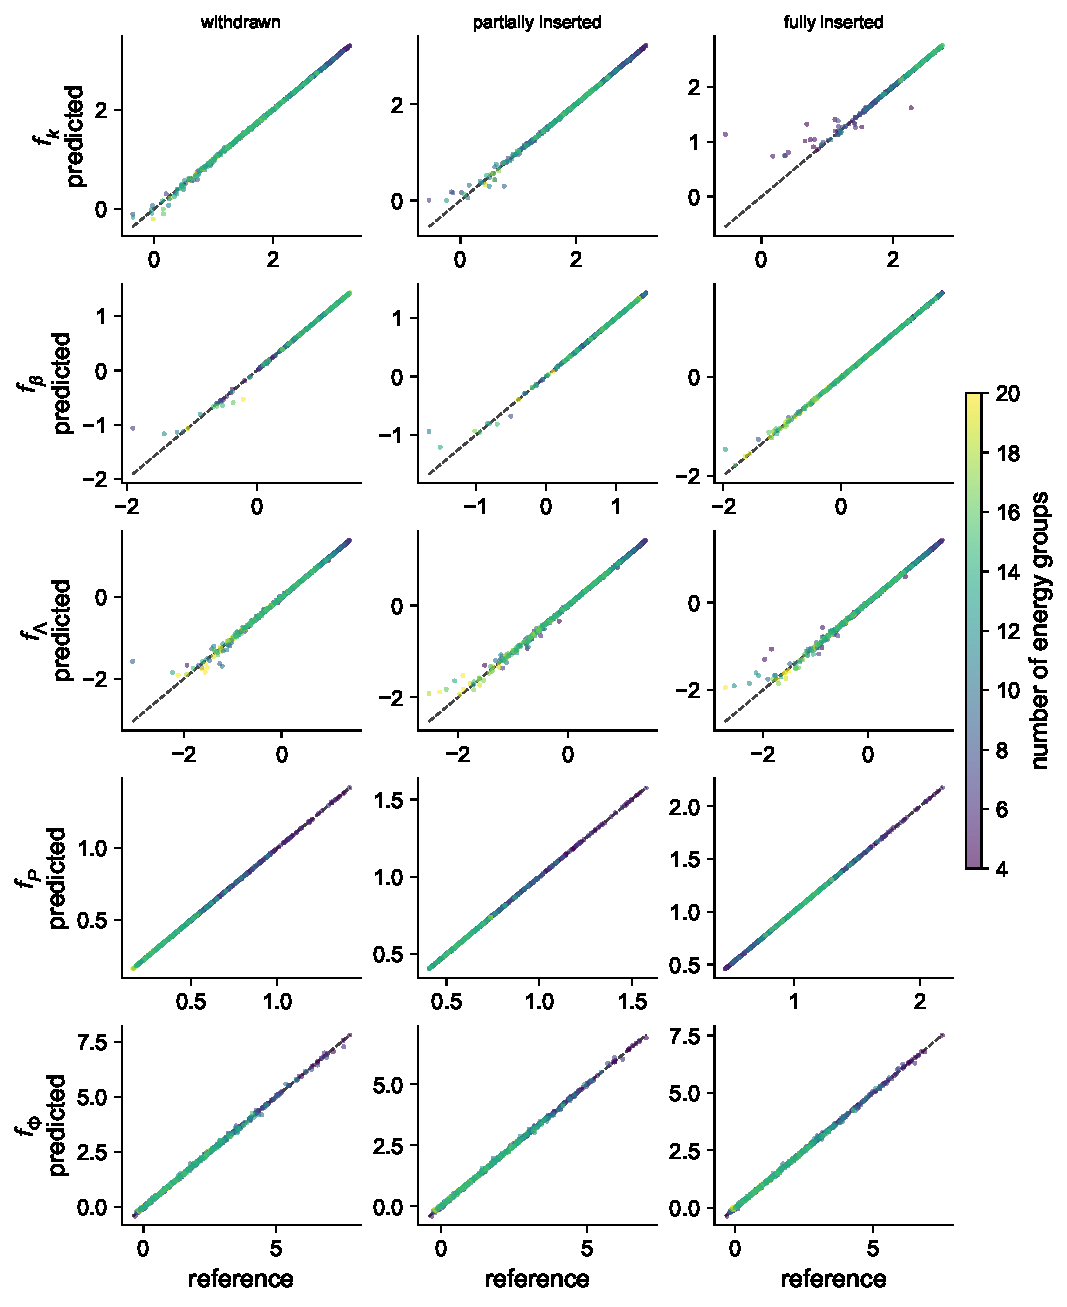
\includegraphics[width=\textwidth]{Chapter4/Figs/fig_scatter.pdf}
  \caption[Predicted against reference values of the fitness functions]{Predicted against reference values of the fifteen fitness functions
  for the 1700 configurations of the external validation set. Rows correspond to
  the five physical families and columns to the three control-rod
  configurations. Colour encodes the number of energy groups of the structure.
  Axes are in the space in which the network is trained, logarithmic for every
  quantity except the power. The dashed line is the identity.}
  \label{eg:fig:scatter}
\end{figure}

The size of the training set was established by a retrospective experiment
rather than assumed. Starting from a random subset of $10\,000$ configurations,
the campaign was replayed by repeatedly training an ensemble, ranking the
remaining configurations by ensemble disagreement and adding the ten thousand
most uncertain ones. The resulting curve, Fig.~\tref{eg:fig:learning}, decreases
steadily and does not flatten before the pool is exhausted, which indicates
that the accuracy is still limited by the amount of available data rather than
by the model. The campaign was stopped because the pool was exhausted, and the
error obtained with the full set is sufficient for the use made of the metamodel
in the following, for the reason set out when the workflow is described.

\begin{figure}[htbp]
  \centering
  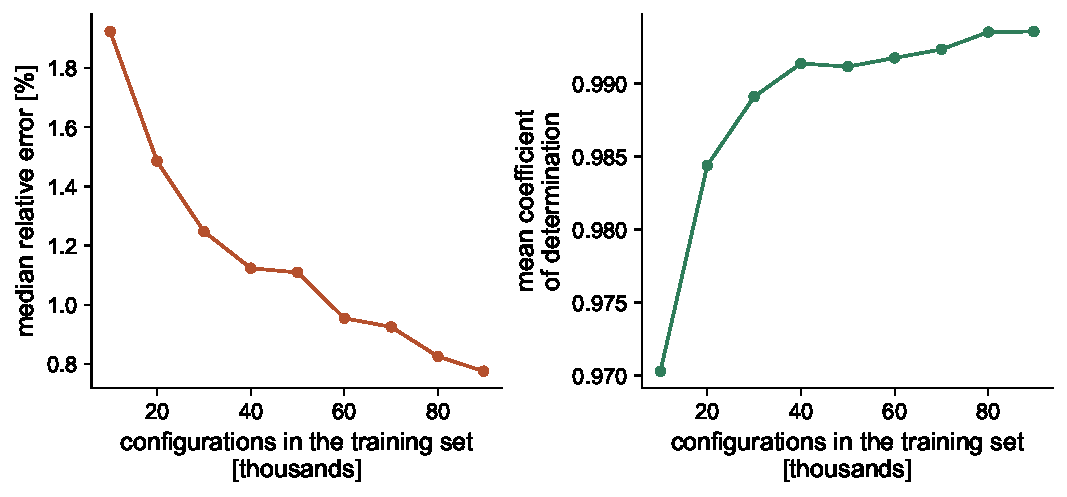
\includegraphics[width=\textwidth]{Chapter4/Figs/fig_learning.pdf}
  \caption[External validation error against the size of the training set]{External validation error as a function of the size of the training
  set, obtained by replaying the acquisition campaign on the assembled data.
  Left, median relative error; right, mean coefficient of determination over the
  fifteen outputs. All the points were obtained with the same reduced training
  protocol, so their absolute level is higher than that of the final ensemble.}
  \label{eg:fig:learning}
\end{figure}

\subsection{The Regime of Reduced Accuracy}

The residual error is not distributed uniformly over the design space. It
concentrates at small values of the reactivity and kinetics fitness functions
and, for the flux, at large values. Since small fitness values identify the best
structures, the behaviour deserves a quantitative explanation, and the
explanation lies in the target function itself. Searching the data set for
pairs of structures differing by exactly one boundary yields 55\,058 such
pairs. The median change of the base-ten logarithm of the fitness function
across a pair amounts to $0.414$ decades in the lowest band of
multiplication-factor deviations, against $0.024$ decades in the highest, a
factor of seventeen, and to $0.395$ against $0.044$ decades for the lifetime.
The correspondence with the accuracy of the metamodel is direct.
Figure~\tref{eg:fig:smallvalue} places the two quantities side by side, band by band
and family by family: where the target changes most under a single boundary
displacement, the metamodel errs most, and the two orderings agree over the
thirty points with a rank correlation of $+0.70$, or $+0.68$ if the flux is
left out. The flux is worth keeping in view because it is the control case: its
steepness grows with the value of the fitness function instead of falling, and
its accuracy degrades in the same direction, opposite to the other four
families. What the error tracks is therefore the local steepness of the target
and not the magnitude of the quantity.

The physical interpretation is direct. A small fitness value means that the
condensed calculation reproduces the Monte Carlo reference almost exactly, and
the comparison with the finest admissible structure, reported further on, shows
how such an agreement is reached:
not by condensing well, but by a cancellation between the error introduced by the
condensation and the error of the deterministic model itself. A cancellation
between two quantities of different origin is fragile, and displacing a single
boundary destroys it. A smooth interpolator cannot follow a function that varies
by half a decade under a one-bit change of its input. This local limitation is
distinct from the aggregate accuracy, which the learning curve shows to be still
limited by the data: more data of the same kind lower the second, not the
first. This is the reason
why the workflow described in the next section does not rely on the metamodel
for its conclusions.

\begin{figure}[htbp]
  \centering
  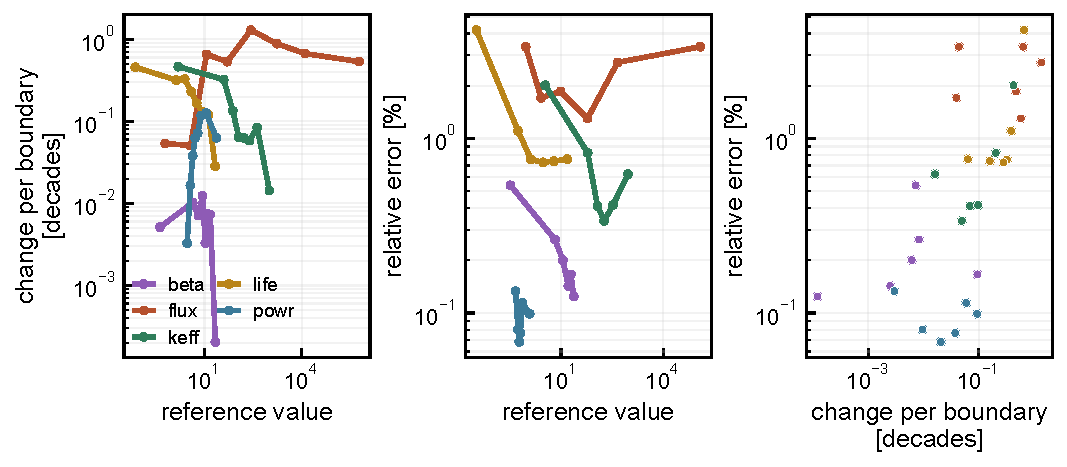
\includegraphics[width=\textwidth]{Chapter4/Figs/fig_steepness.pdf}
  \caption[Steepness of the target and the error of the metamodel]{Left, steepness of the target measured on the pairs of structures
  that differ by exactly one boundary, as the median change of the base-ten
  logarithm of the fitness function across a pair. Centre, median relative error
  of the metamodel over the same bands of the reference value. Right, the two
  quantities plotted against each other, one point per band and family. Colour
  identifies the family, and the axes are logarithmic throughout.}
  \label{eg:fig:smallvalue}
\end{figure}


\section{Workflow}

\subsection{The Scale of the Joint Fitness}

The scaling of Eq.~(\ref{eg:eqn:scaling}) maps each fitness function onto $[1,100]$
using the smallest and the largest value encountered so far in the run. The
choice makes the comparison internally consistent within a generation, since the
population is ranked against its own extremes, but it ties the scale to how much
that particular run has explored. Within a run the scale moves as new extremes
appear, so the joint fitness of an individual is not the same number at
generation ten and at generation ninety, and the formulation compensates by
re-evaluating the whole population at every generation before the survivors are
selected. Between runs the scales are simply different, so the final values are
not comparable at all: a search of 500 generations reports a final fitness
worse than one of 300 generations on the same problem, for no other reason than
having widened its own window.

The search itself is left as it stands. The moving scale, with the
re-evaluation of the population at every generation, is the formulation of
\citet{prevMulti}, and the genetic algorithm optimizes exactly that objective.
What this work adds is a second step, taken after the searches have ended. The
comparison of a thousand independent searches requires a single axis, and it is
obtained by replacing the two extremes of Eq.~(\ref{eg:eqn:scaling}) with the
smallest and the largest value that each fitness function has taken over
everything the thousand searches evaluated, and by re-expressing every outcome
on that window. The window is a property of the campaign as a whole, and since
the searches are mutually independent and already complete when it is built, it
cannot have influenced what any of them found. This common scale, and the
fitness values expressed through it, are referred to as canonical in the
following; the ranking of the candidates, the curve at constrained group count
and every comparison reported below are made on it.

The two ends of the window are not of the same kind. The upper end is a genuine
extreme of what the searches explored, so that a structure would have to be
worse than anything they evaluated to exceed one hundred. The lower end is, for
twelve of the fifteen functions, the threshold of the controls rather than the
smallest value observed, since the searches evaluate structures that reach every
threshold: only the three power functions, to which no control is applied,
begin at a value read from the data. Reaching unity therefore does not require
a structure better than every other evaluated, but only one better than the
threshold, and Sec.~\ref{eg:sec:active} reports which of the fifteen terms end
there. Strictly below unity a controlled term cannot fall, since the control
raises to the threshold every value that would go there; only the three power
functions could, and that would take a structure better than any evaluated by
the campaign.

Whether the window built in this way is an arbitrary choice was measured rather
than assumed, in two ways. The same window computed over the $89\,723$
configurations of the training database, a set the searches never see, assigns
to each of the fifteen functions a width that differs from the one built from
the searches by at most $3\%$; ranked with the two windows, the 747 structures
analysed in the following give a rank correlation of $0.9999$, the same best
structure and the same fifty best. The range that the searches explore on their
own is therefore the range of the problem. Secondly, the whole campaign was
repeated with that fixed window placed inside the search, so that the algorithm
optimizes the canonical fitness directly instead of its own moving scale. The
thousand searches so driven converge to the same best structure, and the
frequencies with which the two campaigns select the 29 boundaries have a rank
correlation of $0.995$; the fixed scale gives a slightly narrower spread of
outcomes, the median search ending $41\%$ above the best against $45\%$, which
is consistent with a stationary objective being marginally easier to optimize
than a moving one, and it runs faster, since the re-evaluation of the population
becomes unnecessary. The formulation of the search was nevertheless kept as
inherited: nothing in the results depends on the choice, and the comparison with
\citet{prevMulti} is then made at equal objective.

\subsection{Multiple Independent Searches}

The searches use a population of 100 individuals over 100 generations, with
tournament selection, two-point crossover, integer random mutation at $0.05$ per
gene and the repair operator introduced with the chromosome. The
implementation is built on the pymoo library~\cite{pymoo} and reproduces the
scheme of \citet{prevMulti} in its representation, operators and fitness
functions. The population and generation counts were established by
measurement: a population of 40 individuals yields a median final fitness $1.7$
times worse and a population of 200 improves it by $17\%$ at twice the cost per
search, while the median search reaches within $1\%$ of its own final value by
generation 36 and 85 searches out of a thousand are still improving after
generation 90. The population was kept at 100 and the budget spent on the number
of independent searches instead, a choice the following section quantifies.

One implementation detail deserves mention because it affects reproducibility.
The sampling and mutation operators of this problem draw from the global random
generator, which the optimization library does not seed, so that the seed passed
to the optimizer has no effect and successive runs are not reproducible.
Seeding the global generator explicitly before each tribe restores bit-level
reproducibility, and all results presented here can be regenerated exactly.

The searches are mutually independent and are executed in parallel. One thousand
of them require $841$~s on fourteen processes, about three core-hours, so that
the cost of exploring the design space a thousand times over is smaller than the
cost of a hundred evaluations of the reference solver.

\subsection{Verification with the Reference Solver}

Every distinct structure produced by the searches is submitted to FRENETIC, and
the ranking reported in the following is the one obtained from the recomputed
values, expressed on the canonical scale. No quantity discussed in the following is a prediction of the metamodel.
This arrangement is deliberate and follows from the limit just characterised:
the metamodel is accurate
enough to order the candidates and thus to identify a short list worth a
full-core calculation, which is a considerably weaker requirement than
predicting the fitness of the best structures to the precision needed to rank
them among themselves.


\section{Results and Discussion}

\subsection{Behaviour of the Searches}

The thousand searches produced 747 distinct structures, with a number of groups
between 9 and 20. Figure~\tref{eg:fig:search} summarises their behaviour, with
the progress of every search re-expressed on the canonical scale. Each search
settles quickly: measured against its own final value, the median search is
within $10\%$ of it by generation 24 and within $1\%$ by generation 36, and 85
searches out of a thousand are still improving after generation 90. Where they
settle is another matter. Two searches out of a hundred end within $5\%$ of the
best structure, a single one out of the thousand reaches it, and the median
search ends $45\%$ above it, so that a single search returns a structure of the
right order but not the best one, and which structure it returns is not
determined by the problem alone. The outcomes
spread over twelve different group counts. This confirms the observation of
\citet{prevMulti} on a sample larger by more than two orders of magnitude, and
the next subsection makes it quantitative.

\begin{figure}[htbp]
  \centering
  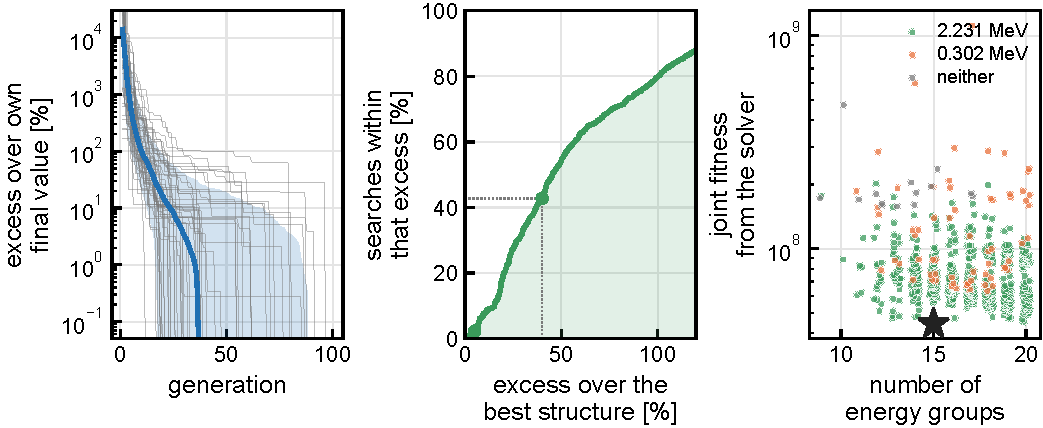
\includegraphics[width=\textwidth]{Chapter4/Figs/fig_search.pdf}
  \caption[Behaviour of the thousand independent searches]{Behaviour of the thousand independent searches. Left, distance of each
  search from its own final value, generation by generation, the best structure
  found so far being re-expressed on the canonical scale, as one faint line
  every twentieth search with the median and the band between the tenth and
  ninetieth percentiles. Centre, fraction of the searches whose outcome lies
  within a given excess over the best structure found, with the values at five
  and forty per cent marked. Right, joint fitness returned by the reference
  solver against the number of groups, one point per distinct structure with a
  small horizontal jitter, coloured by the choice made in the fast region and
  with the best structure starred.}
  \label{eg:fig:search}
\end{figure}

The internal dynamics of a single search are illustrated in
Fig.~\tref{eg:fig:tribe}. The initial population is heterogeneous, most boundaries
being present in about half of the individuals, and within a dozen generations
the population crystallises, each boundary being either adopted by nearly every
individual or abandoned by nearly all of them. Later events, in which a boundary
that had been fixed is re-opened and replaced, show that crossover and mutation
continue to restructure the solution after the joint fitness has apparently
settled.

\begin{figure}[htbp]
  \centering
  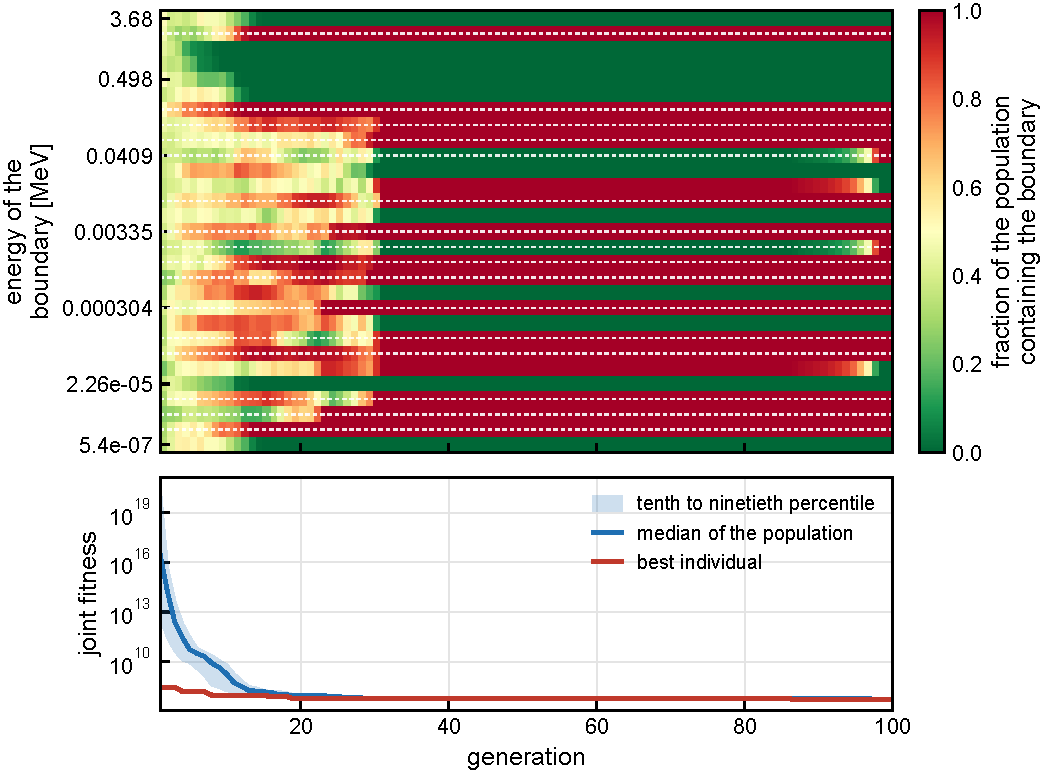
\includegraphics[width=\textwidth]{Chapter4/Figs/fig_tribe.pdf}
  \caption[Evolution of a single search]{Evolution of a single search. Above, fraction of the population
  containing each internal boundary, generation by generation, from green when
  the boundary is absent from the whole population to red when every individual
  carries it, the white dotted lines marking the boundaries of the final
  structure of this search. Below, on the same generation axis, joint fitness of
  the population as the band between the tenth and ninetieth percentiles, its
  median and the best individual.}
  \label{eg:fig:tribe}
\end{figure}

\subsection{How Many Searches Are Enough}\label{eg:sec:howmany}

The size of the campaign was not chosen a priori, and the same data allow it to
be justified after the fact by re-drawing subsets of the thousand outcomes at
random. The question has three answers depending on what is asked of the sample,
and Fig.~\tref{eg:fig:howmany} separates them.

The first concerns the optimum, and it is the result that motivates this work.
Table~\tref{eg:tab:howmany} reports how close the best of $n$ searches comes to
the best of the thousand. A single search lands $45\%$ above it, and three
searches, which is what a campaign with the reference solver inside the loop can
afford, land $20\%$ above; ten searches reach $9\%$, thirty reach $5\%$ and a
hundred reach $2\%$, which is the distance of the second-best structure: the
best one was returned by a single search out of the thousand, so that even a
hundred searches typically stop at the second. Read the other way, the
probability of landing within $5\%$ of the best structure is $2\%$ for one
search, $7\%$ for three and $92\%$ for a hundred. The gain from repeating the search is therefore neither marginal nor
unbounded: it is concentrated between one search and a few tens of them, and it
is precisely the range that the reference solver cannot reach and the metamodel
can.

\begin{table}[htbp]
\centering
\caption[Effect of the number of independent searches]{Effect of the number of
independent searches, obtained by drawing subsets of the thousand outcomes at
random. The excess is measured on the values returned by the reference solver,
against the best structure of the whole campaign.}
\label{eg:tab:howmany}
\begin{tabular}{rcc}
\toprule
Searches & Median excess over the best & Within $5\%$ of the best \\ \midrule
    1    & \SI{45}{\percent} & \SI{2}{\percent} \\
    3    & \SI{20}{\percent} & \SI{7}{\percent} \\
    10   & \SI{9}{\percent}  & \SI{20}{\percent} \\
    30   & \SI{5}{\percent}  & \SI{50}{\percent} \\
    100  & \SI{2}{\percent}  & \SI{92}{\percent} \\
    1000 & \SI{0}{\percent}  & \SI{100}{\percent} \\
\bottomrule
\end{tabular}
\end{table}

The second concerns the regularities of the optimized structures, and here the
sample is more than sufficient. What those regularities rest on is the
frequency with which each of the 29 boundaries is selected, and a hundred
searches already fix every one of those frequencies to within ten points of the
value obtained from the thousand, and to within three points for the typical
boundary; three hundred searches bring the worst case to six points. More
searches narrow those margins, but they cannot add boundaries to the parent
mesh, which is what would add anything new to the comparison.

The third question is the one the sample does not answer, and the right panel of
Fig.~\tref{eg:fig:howmany} shows it plainly: the number of distinct structures is
still growing at the thousandth search. Of the 747 structures obtained, 619 were
produced by exactly one search, so that five structures out of six have been
seen once, which is what a sample far from complete looks like. A further search
returns a structure already obtained in about four cases out of ten. A complete
census of the reachable structures is out of reach, and no claim of that kind is
made here. The situation is that of a fisherman who sets out to take a census
of the species of the sea from what his net brings up. As long as nearly every
haul brings a species not seen before, each haul adds to what is known, but it
also says that the census is far from complete; only when the same species keep
returning, haul after haul, can the census be considered close to exhaustive.
Here six hauls out of ten still bring a species never seen before.

What is missing, however, is missing for a reason that limits the damage. A
structure absent from the sample is one the algorithm reaches rarely, and the
rate at which it is reached is related to its quality: the 619 structures
produced by a single search have a median true fitness $25\%$ worse than the 128
produced by more than one. The unseen part of the population is expected to
consist mostly of the poorer attractors, which is the part that matters least
for the conclusions drawn here.

\begin{figure}[htbp]
  \centering
  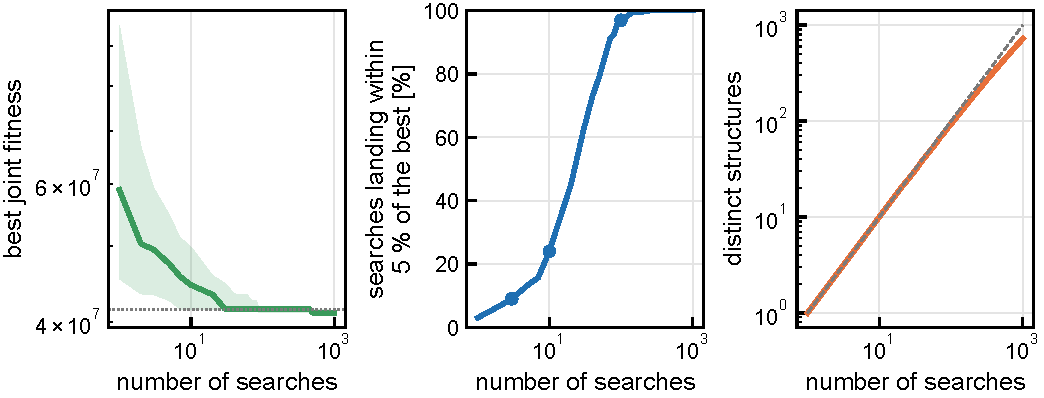
\includegraphics[width=\textwidth]{Chapter4/Figs/fig_howmany.pdf}
  \caption[Effect of the number of independent searches]{Effect of the number of independent searches, obtained by re-drawing
  subsets of the thousand outcomes at random. Left, best joint fitness reached,
  with the band between the tenth and ninetieth percentiles and the dotted line
  one per cent above the value of the whole campaign. Centre, fraction of the
  draws whose best structure lies within five per cent of the best of the
  campaign, with the values at three, ten and a hundred searches marked. Right,
  number of distinct structures obtained, against the dashed line that would be
  reached if every search returned a different one.}
  \label{eg:fig:howmany}
\end{figure}

\subsection{The Choice in the Fast Region}\label{eg:sec:families}

The 747 structures are not distributed freely over the pool of boundaries: one
choice in the fast region is taken by almost all of them, and it excludes
another. No structure among the 747 retains both the boundary at $2.231$ and the
one at $0.302$~MeV. The exclusion is complete, and it is not the consequence of
a preference for one of the two, since 14 structures retain neither: the two
boundaries are alternative, and the alternative is decided in favour of the
first in $89\%$ of the cases against $9\%$ for the second.

That choice carries others with it. Among the structures that adopt
$2.231$~MeV, $90\%$ also adopt the boundary at $4\times10^{-6}$~MeV, which
appears in $2\%$ of those that adopt $0.302$~MeV; conversely, $83\%$ of the
latter adopt $3.679$~MeV and the thermal cut at $5.4\times10^{-7}$~MeV, against
$20$ and $21\%$ of the former. The two blocks are therefore coherent well beyond
the boundaries that define them, and Table~\tref{eg:tab:families} reports the
frequencies.

The exclusion has a direct reading. The boundaries at $3.679$ and $2.231$~MeV
are adjacent in the fine mesh, so that retaining both would subdivide a region
which carries $1.6\%$ of the flux and $0.3\%$ of the importance, and
once one of the two is adopted the placement of the remaining boundaries adapts
to it. Crossing from one block to the other means removing one boundary and
adding another, and no single mutation performs the passage, which is why a
search remains within the block in which its initial population happens to fall.

The two blocks are not equivalent, and the imbalance in their populations is
matched by a difference in quality. The 668 structures that adopt $2.231$~MeV
have a median true fitness of $6.70\times10^{7}$ against $9.96\times10^{7}$ for
the 65 that adopt $0.302$~MeV, and the best structure of the first block is
better than the best of the second by more than forty per cent. The fourteen
structures that adopt neither boundary are worse than the first block by a
factor of $2.7$ in median fitness and than the second by $1.8$, which confirms that one of the two is needed and that the
search is choosing between two ways of covering the same region rather than
deciding whether to cover it.

Which of the two prevails is not explained by the fidelity with which each
represents the spectrum, and the point is worth recording because the opposite
would be the natural expectation. For each structure the variation of the
reference flux shape within its groups was computed and weighted by the total
importance $\phi\phi^{\ddagger}/v$ of the group, which is the weight with which
the flux fitness function of Eq.~(\ref{eg:eqn:distributed}) counts an error. The
two blocks are indistinguishable on that measure, $0.171$ against $0.159$, and
they remain so when the weight is the bare flux, $0.237$ against $0.252$. The
separation into two blocks is a property of the solutions, and the difference in
quality between them is measured here; what decides it is not identified by
these data.

\begin{table}[htbp]
\centering
\caption[The two blocks of solutions]{The two blocks of solutions, defined by
the exclusive choice between the boundaries at $2.231$ and $0.302$~MeV. Above,
the boundaries whose presence distinguishes them, with the fraction of the
structures of each block that retains the boundary. Below, the properties of the
two blocks: the median joint fitness verified with the reference solver, the
mean number of boundaries on which two structures of the same block disagree,
and the variation of the reference flux shape within the groups, weighted by the
total importance that appears in the flux fitness function and, for comparison,
by the bare flux. Two structures belonging to different blocks disagree on
$12.5$ boundaries on average.}
\label{eg:tab:families}
\small
\begin{tabular}{lcc}
\toprule
Boundary [MeV] & $2.231$~MeV block [\%] & $0.302$~MeV block [\%] \\ \midrule
    $2.231$ & 100 & 0 \\
    $3.020\times10^{-1}$ & 0 & 100 \\
    $4.000\times10^{-6}$ & 90 & 2 \\
    $3.679$ & 20 & 83 \\
    $5.400\times10^{-7}$ & 21 & 83 \\
    $9.166\times10^{-5}$ & 57 & 3 \\
\midrule
    Property & $2.231$~MeV block & $0.302$~MeV block \\ \midrule
    Distinct structures & 668 & 65 \\
    Median joint fitness & $6.700\times10^{7}$ & $9.956\times10^{7}$ \\
    Mean internal disagreement [boundaries] & 9.1 & 7.3 \\
    Shape variation, importance weighted & 0.171 & 0.159 \\
    Shape variation, flux weighted & 0.237 & 0.252 \\ \bottomrule
\end{tabular}
\end{table}

\subsection{Recurring Features of the Optimized Structures}\label{eg:sec:recurring}

Beyond the choice just described, the 747 structures display regularities which
can be examined collectively, and which constitute the general information that
a single search cannot provide.

Table~\tref{eg:tab:boundaries} reports, for each of the 29 internal boundaries of
the fine mesh, how often it is retained. The distribution is broad, and no
boundary is common to the solutions: the most frequent, at $0.183$~MeV, appears
in $96\%$ of the structures, the next two, at $8.3\times10^{-6}$ and
$2.231$~MeV, in $91$ and $89\%$, while no other exceeds $87\%$. At the other
end four boundaries are used by fewer than one structure in ten, all of them in
the fast region between $0.30$ and $1.35$~MeV. The optimized structures
therefore agree on very little, and two of them taken at random disagree on
$9.7$ of the 29 boundaries.

\begin{table}[htbp]
\centering
\caption[The 29 internal boundaries of the fine mesh]{The 29 internal boundaries
of the fine mesh. For each one: the fraction of the 747 distinct optimized
structures that retains it, the mean share of the total importance
$\phi\phi^{\ddagger}/v$ carried by the two groups it separates, evaluated on the
reference calculation with the rods partially inserted, and whether it belongs
to the best structure found.}
\label{eg:tab:boundaries}
\small
\setlength{\tabcolsep}{4pt}
\begin{tabular}{rccc@{\hspace{4mm}}rccc}
\toprule
$E$ [MeV] & Occ.\ [\%] & Imp.\ [\%] & Best &
$E$ [MeV] & Occ.\ [\%] & Imp.\ [\%] & Best \\ \midrule
    $3.68$ & 25 & 0.2 &  & $2.03\times10^{-3}$ & 78 & 5.7 & $\bullet$ \\
    $2.23$ & 89 & 0.4 & $\bullet$ & $1.23\times10^{-3}$ & 69 & 5.3 & $\bullet$ \\
    $1.35$ & 0 & 0.8 &  & $7.49\times10^{-4}$ & 76 & 4.4 &  \\
    $8.21\times10^{-1}$ & 2 & 1.8 &  & $4.54\times10^{-4}$ & 45 & 3.2 & $\bullet$ \\
    $4.98\times10^{-1}$ & 0 & 2.7 &  & $3.04\times10^{-4}$ & 87 & 3.3 & $\bullet$ \\
    $3.02\times10^{-1}$ & 9 & 3.4 &  & $1.49\times10^{-4}$ & 21 & 3.5 &  \\
    $1.83\times10^{-1}$ & 96 & 4.5 & $\bullet$ & $9.17\times10^{-5}$ & 51 & 2.1 &  \\
    $1.11\times10^{-1}$ & 66 & 5.1 & $\bullet$ & $6.79\times10^{-5}$ & 45 & 2.0 &  \\
    $6.74\times10^{-2}$ & 70 & 5.3 &  & $4.02\times10^{-5}$ & 37 & 2.4 &  \\
    $4.09\times10^{-2}$ & 58 & 5.3 &  & $2.26\times10^{-5}$ & 48 & 2.3 & $\bullet$ \\
    $2.48\times10^{-2}$ & 66 & 5.4 & $\bullet$ & $1.37\times10^{-5}$ & 77 & 2.1 & $\bullet$ \\
    $1.50\times10^{-2}$ & 59 & 5.7 &  & $8.32\times10^{-6}$ & 91 & 2.1 &  \\
    $9.12\times10^{-3}$ & 62 & 5.3 & $\bullet$ & $4.00\times10^{-6}$ & 82 & 2.4 & $\bullet$ \\
    $5.53\times10^{-3}$ & 69 & 5.2 & $\bullet$ & $5.40\times10^{-7}$ & 26 & 1.9 &  \\
    $3.35\times10^{-3}$ & 74 & 5.5 & $\bullet$ &  & & &  \\
\bottomrule
\end{tabular}
\end{table}


The placement of the recurring boundaries admits a physical reading which is not
the one that intuition suggests. A natural expectation is that boundaries should
be placed where the spectrum changes shape most abruptly, since a single group
cannot represent a rapidly varying flux, and that they should follow the flux
itself, since a group carrying little flux contributes little to the reaction
rates. The structures say otherwise. The three boundaries of the fast region
where the spectrum bends most sharply, at $1.35$, $0.821$ and $0.498$~MeV, are
used by at most one structure in fifty, although the region they subdivide,
between $2.231$ and $0.302$~MeV, carries $23\%$ of the flux; and
Fig.~\tref{eg:fig:boundaries}, which sets the selection frequency against the
importance surrounding the boundary and against the variation of the flux shape
across it, shows nothing that twenty-nine points would allow to call a trend
with either quantity. What the figure does show is where the two readings part
company, which is the fast region, and the reason is physical. The flux fitness
function of Eq.~(\ref{eg:eqn:distributed}) measures the flux error of every
group weighted by the total importance $\phi\phi^{\ddagger}/v$, so that the
relevant measure of how much a group matters is not how much flux it carries
but how much importance it carries. The adjoint flux of this core varies by less
than a factor of two over the whole energy range, so the importance follows
essentially the ratio $\phi/v$: the fast groups carry a substantial part of the
flux but, at those speeds, only a small part of the importance, the ratio
between the two fractions rising from $0.14$ in the highest group to unity
around $10$~keV. The optimizer places its boundaries according to the second
quantity and not the first, and the two regions of the spectrum show it. Above
$0.3$~MeV the groups on either side of a boundary carry between $0.2$ and
$2.7\%$ of the importance, and the structures keep a single boundary there and
drop the other four; between $0.18$~MeV and $0.75$~keV they carry between $4.4$
and $5.7\%$, an almost flat plateau, and there every boundary is retained by
more than half of the structures.

The tendency can be stated more directly, and in this form it separates the two
readings without ambiguity. Computing for each structure the coefficient of
variation of the importance contained in its groups gives $0.573$ for the ten
best structures against $0.856$ for random structures with the same number of
groups, so that the optimized structures distribute the importance $1.5$ times
more evenly. The same measure applied to the bare flux gives $1.387$ against
$1.218$: on that quantity the optimized structures are not more even than random
ones but less. The optimization therefore moves towards an equipartition of the
importance among the groups, and away from an equipartition of the flux, a
criterion which was never imposed explicitly and which follows from the
weighting of Eq.~(\ref{eg:eqn:distributed}).

\begin{figure}[htbp]
  \centering
  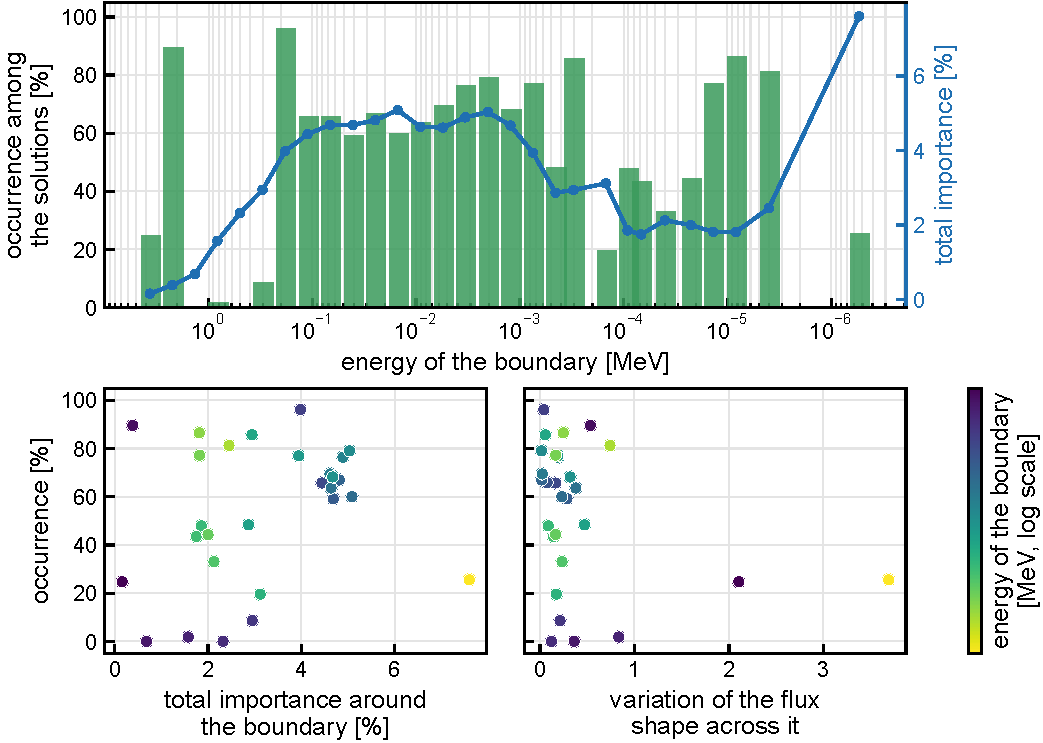
\includegraphics[width=\textwidth]{Chapter4/Figs/fig_boundaries.pdf}
  \caption[Recurring features of the optimized structures]{Recurring features of the optimized structures. Above, frequency with
  which each internal boundary is selected among the 747 distinct structures,
  each bar coloured by the energy of its boundary, and total importance
  surrounding each boundary on the same energy axis, in blue. Below, the same
  frequency plotted against the surrounding importance and against the variation
  of the flux shape across the boundary, with the same colour scale for the
  energy of the boundary.}
  \label{eg:fig:boundaries}
\end{figure}


\subsection{Number of Groups}

Repeating the optimization with the number of groups constrained, on the
canonical scale, gives the fitness attainable as a function of $G$, shown in
Fig.~\tref{eg:fig:tradeoff} with every point verified by FRENETIC. The attainable
fitness improves by a factor of $4.2$ between $G=8$ and the minimum, which falls
at $G=15$ and coincides with the best structure of the unconstrained campaign,
and it is essentially flat over a wide range: six of the group counts between
$G=12$ and $G=20$ lie within $10\%$ of that minimum. Twelve groups are therefore sufficient for this core and this set
of fitness functions, and the additional groups used by the best structures
bring little further benefit. The curve is not monotone inside the basin,
reaching $5.5\times10^{7}$ at $G=16$ against $4.4\times10^{7}$ at $G=15$: each
point is the best structure a constrained search found at that group count, so
the curve is an upper bound on the attainable fitness and the residual roughness
measures how hard the search is at fixed $G$, not a feature of the landscape.
Seventeen constrained optimizations of this kind require two minutes on the
metamodel and would require of the order of six thousand core-hours on the
solver.

\begin{figure}[htbp]
  \centering
  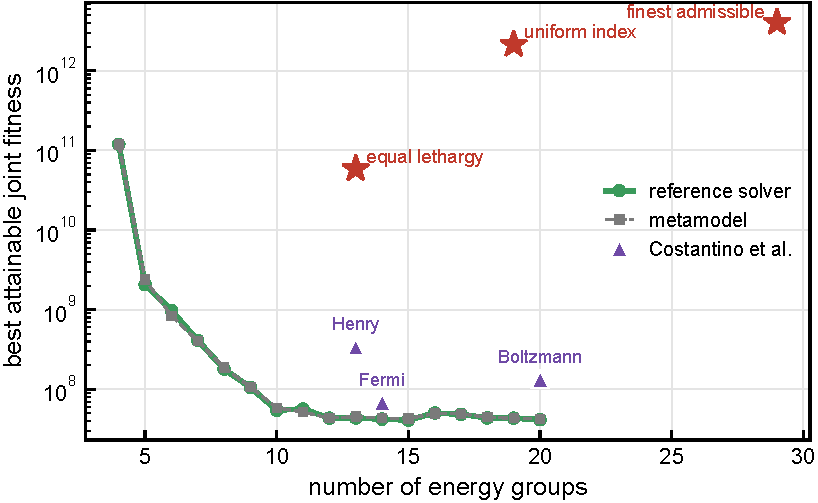
\includegraphics[width=0.79\textwidth]{Chapter4/Figs/fig_tradeoff.pdf}
  \caption[Best attainable joint fitness against the number of groups]{Best attainable joint fitness as a function of the number of energy
  groups, obtained by repeating the searches with the group count constrained.
  Each point of the solid curve was verified with the reference solver, while
  the dashed curve is the corresponding prediction of the metamodel. The faded
  blue points are the 747 distinct structures returned by the thousand
  unconstrained searches, placed at their own group count with a small
  horizontal jitter, and mark the region the campaign actually visited. The
  stars mark the reference constructions discussed in the text, and the
  triangles the structures obtained by the three tribes of \citet{prevMulti},
  recomputed here on the same canonical scale.}
  \label{eg:fig:tradeoff}
\end{figure}

\subsection{Comparison with Reference Structures}

The best verified structure uses $G=15$ groups and reaches a canonical fitness
of $4.4319\times10^{7}$. Its fourteen internal boundaries are marked in the last
column of Table~\tref{eg:tab:boundaries}: it adopts the boundary at $2.231$~MeV
and therefore belongs to the block that prevails, it uses none of the four
boundaries that the searches almost never select, and it does not contain the
boundary at $8.3\times10^{-6}$~MeV that nine structures out of ten retain, so
that not even the most frequent boundaries are indispensable. It outperforms every one of
the $124\,693$ configurations computed to date, by $28\%$ with respect to the
best among them, and none of those configurations reaches its fitness.

The comparison that matters most is with the three tribes of
\citet{prevMulti}, whose structures are the outcome of the same problem
solved with the reference solver inside the loop, and which were recomputed here
on the canonical scale from the boundaries reported in that work. They are shown
in Fig.~\tref{eg:fig:tradeoff} together with the curve of the best attainable
fitness, and they lie above it: at $G=14$ the best of the three reaches
$7.37\times10^{7}$ against $4.55\times10^{7}$ attainable, at $G=20$
$1.45\times10^{8}$ against $4.53\times10^{7}$, and at $G=13$ $3.60\times10^{8}$
against $4.92\times10^{7}$. The gap, between $1.6$ and $7.3$ times at equal
group count, is a question of how many searches were affordable, and the
outcomes of the thousand searches, shown as the faded cloud in the same figure,
say so directly: the three structures fall inside the region the campaign
visits, not outside it. At $G=14$ the structure of \citet{prevMulti} is a
typical outcome of one of our searches, worse than 24 of the 57 structures the
campaign returned at that group count and better than the other 33; at $G=20$ it
lies in the upper tail, worse than 95 of 101; at $G=13$ it is worse than all 37.
None of them is unreachable by a single search, and none is what a single search
is likely to return. With the reference solver inside the loop, three tribes
were what a reasonable budget allowed, and the same three tribes are the reason this chapter exists, since it
was their disagreement that first showed the outcome to depend on the seed. The
objective is the same in the two cases, so the comparison measures the size of
the campaign and nothing else.

Table~\tref{eg:tab:standard} compares the optimized structure with three further
reference constructions. A structure with uniformly spaced boundary indices and
nineteen groups is worse by a factor of $5.0\times10^{4}$, and one with uniform
lethargy spacing by a factor of $1.4\times10^{3}$. It is worth noting that a
uniform-lethargy structure cannot be built with 19 boundaries on this fine mesh,
since the 30 fine groups are not themselves equally spaced in lethargy, so that
equally spaced targets collapse onto repeated boundaries and only 13 survive.
The fine mesh constrains which regular structures can be constructed at all.

\begin{table}[htbp]
\centering
\caption[The optimized structure against three reference ones]{The optimized
structure against three reference ones, quantity by quantity: two built with
standard spacing rules and the finest structure the collapsing procedure admits,
obtained by suppressing a single boundary of the fine mesh. Each entry is the
scaled contribution entering the joint fitness, obtained from the FRENETIC
values through the fixed canonical window: unity is the lower end of that
window, which any term already at the threshold of the controls attains, and 100
the upper end.}
\label{eg:tab:standard}
\begin{tabular}{lcccc}
\toprule
Figure of merit & Optimized & Equal & Uniform & Finest \\
     &  & lethargy & index & admissible \\
    $G$ & 15 & 13 & 19 & 29 \\ \midrule
    $f_{k,\mathrm{out}}$ & 6.7 & 1.0 & 3.2 & 7.2 \\
    $f_{k,\mathrm{partial}}$ & 1.0 & 7.2 & 9.6 & 14.2 \\
    $f_{k,\mathrm{in}}$ & 61.6 & 72.6 & 74.5 & 86.5 \\
    $f_{\beta,\mathrm{out}}$ & 1.0 & 52.3 & 82.9 & 98.9 \\
    $f_{\beta,\mathrm{partial}}$ & 1.0 & 19.0 & 51.3 & 68.0 \\
    $f_{\beta,\mathrm{in}}$ & 21.4 & 1.0 & 1.0 & 1.0 \\
    $f_{\ell,\mathrm{out}}$ & 1.0 & 2.1 & 2.3 & 1.3 \\
    $f_{\ell,\mathrm{partial}}$ & 2.2 & 1.5 & 2.4 & 1.0 \\
    $f_{\ell,\mathrm{in}}$ & 1.0 & 4.3 & 3.6 & 4.6 \\
    $f_{P,\mathrm{out}}$ & 6.1 & 14.8 & 16.0 & 15.6 \\
    $f_{P,\mathrm{partial}}$ & 10.7 & 15.6 & 17.9 & 18.7 \\
    $f_{P,\mathrm{in}}$ & 34.0 & 38.2 & 39.8 & 40.8 \\
    $f_{\Phi,\mathrm{out}}$ & 1.0 & 1.0 & 1.0 & 1.0 \\
    $f_{\Phi,\mathrm{partial}}$ & 1.0 & 1.0 & 1.0 & 1.0 \\
    $f_{\Phi,\mathrm{in}}$ & 1.0 & 1.0 & 1.0 & 1.0 \\
\midrule
    Joint fitness & $4.432\times10^{7}$ & $6.042\times10^{10}$ & $2.211\times10^{12}$ & $4.205\times10^{12}$ \\
\bottomrule
\end{tabular}
\end{table}


The third reference is the finest structure the framework admits. The collapsing
routine requires the condensed structure to contain fewer groups than the fine
one, so that $G=30$ is not a legitimate option and the limit is $G=29$, obtained
by suppressing a single boundary. All twenty-nine such structures were
evaluated. The best of them, obtained by suppressing the boundary at
$8.3\times10^{-6}$~MeV, reaches a canonical fitness of $4.20\times10^{12}$, the
median is $6.81\times10^{13}$ and the worst is $7.25\times10^{16}$.

The optimized 15-group structure is therefore better than the best 29-group
structure by five orders of magnitude on the joint fitness. Since that fitness
is a product of fifteen scaled terms, the factor compounds differences which are
individually moderate, and it is instructive to look at the terms one by one in
Table~\tref{eg:tab:standard}. The finest structure is better than the optimized
one on two of the fifteen quantities, the delayed neutron fraction and the
lifetime in one configuration each, and worse on the other thirteen. Where it
loses most is on the integral parameters: the deviation on the multiplication
factor with the rods partially inserted is $239$~pcm against $9.6$~pcm, and the
deviation on the delayed neutron fraction in the same configuration is $21.6$
against $2.0$~pcm.

The interpretation is that these residual deviations are not caused by the
energy mesh. A 29-group structure condenses almost nothing, so what remains is
the error of the deterministic model itself, namely the diffusion approximation
and the spatial homogenization, measured against a Monte Carlo reference that
contains neither. The optimization cannot remove that error, but it can offset
it: a coarser structure introduces a condensation error of its own, and the
search selects the structure whose condensation error cancels the model error
most closely. The fifteen-group structure reproduces the multiplication factor
with the rods partially inserted almost exactly not because it condenses better,
but because its condensation error and the model error very nearly cancel.

Two consequences follow. The first is practical: refining the energy mesh is not
a way of approaching the Monte Carlo reference in this framework, and a
carefully chosen coarse structure is worth more than the finest admissible one,
which is the strongest justification for optimizing the structure at all. The
second concerns the metamodel: since the best structures owe their quality to a
cancellation between two errors of different origin, their fitness is bound to
be a fragile function of the mesh, and therefore a hard one to interpolate.

A third consequence concerns the scope of the result, and is worth stating
plainly because it was so far left implicit. If the quality of a structure rests
on a cancellation, the structure is bound to everything that fixes the two
errors being cancelled. It is specific to the core analysed, with its geometry,
its materials and its enrichments, and to the operating states over which the
search was conducted, the three control-rod configurations at the single
isothermal state point at which the reference data were generated. It is
specific to the deterministic scheme whose error it offsets, the diffusion
approximation together with the assembly-wise homogenization: it would not
offset the error of a transport solver, nor that of a different homogenization.
It is specific to the reference against which the agreement is measured, and to
the precision of that reference, which enters the objective directly through the
clipping of the three integral fitness functions, whose thresholds are set a few
times above the statistical uncertainty of that reference. It is specific to the
objective itself, in the five quantities chosen and equally in the way they are
combined by Eq.~(\ref{eg:eqn:joint}), since the clipping and the logarithm decide
which deviations the search is still allowed to see. And it is confined to the
pool it was offered, the boundaries of the 30-group parent mesh, outside which
no search can place a cut.

None of this weakens the result, but it delimits it: what carries over to
another core, another solver or another set of target quantities is the
procedure, not the fourteen boundaries it produced here. The point runs against
the intuition that a better structure should also be a more general one, and the
cancellation is precisely the reason why the opposite holds: the closer a
structure comes to the reference, the more tightly it is tied to the particular
pair of errors it was tuned to annul.

\subsection{Which Terms of the Fitness Are Active}\label{eg:sec:active}

Not every term of Eq.~(\ref{eg:eqn:joint}) takes part in the ranking of the
optimized structures. Evaluating the fifteen scaled terms for each of the 747
verified structures shows that three of them sit at the minimum of the canonical
window for every one: the flux with the rods withdrawn and partially inserted,
and the delayed neutron fraction with the rods partially inserted. Two more are
there for almost every structure, the delayed neutron fraction with the rods
withdrawn in 732 cases out of 747 and the flux with the rods fully inserted in
745.

The two groups do not share a cause. The delayed neutron fraction is held at the
minimum by the clipping applied before the scaling, in the sense for which the
control was introduced: the quantity is reproduced to within ten pcm, is
clipped, and stops contributing to the ranking, so that the search is directed
towards what is still worth improving. The three flux terms are held there by
the logarithmic floor, which corresponds to a weighted relative error of ten
and which no optimized structure approaches, the best reaching values between
$1.0$ and $1.3$. That floor
is inherited with the formulation of \citet{prevMulti} and it is retained here
unchanged, so that the flux takes no part in the ranking among the optimized
structures. It bounds what the optimization can be said to have achieved on that
quantity, and it is stated for that reason.

Ten terms therefore discriminate, against the five that do not, and the joint
fitness of a good structure is effectively a product of ten factors. The
quantity on which the metamodel is least accurate in relative terms, the
lifetime with the rods withdrawn, is clipped for most of these structures, which
reproduce it to a few thousandths of a per cent: its relative error is large
because the quantity is small, and the corresponding absolute error lies below
the statistical uncertainty of the reference.

\subsection{Accuracy of the Metamodel on the Proposed Structures}\label{eg:sec:accuracy}

All 747 distinct structures were recomputed with FRENETIC, which allows the
metamodel to be judged on exactly the population it proposed and on the
quantity the search actually uses, the joint fitness. The median difference
between the predicted and the true joint fitness over the 747 structures is
$2.0\%$ and the rank correlation between the two is $0.990$, while the accuracy
on the fifteen quantities themselves is $0.39\%$, the same as on the external
validation set. The structure that the metamodel ranks first is the second
according to the solver, $2.3\%$ behind the first, and the first according to
the solver is the second of the metamodel, so that verifying the three best
candidates of the metamodel is enough to recover the best structure. This is
the property the workflow needs: the ordering produced by the metamodel
reproduces the ordering of the solver closely enough that a search driven by
predictions arrives in the same region of the design space as a search driven
by the solver would, and the verification of every structure the searches
produce settles the rest. The fifteen best structures are listed in
Table~\tref{eg:tab:ranking}.

\begin{table}[htbp]
\centering
\caption[The fifteen best of the 747 distinct structures]{The fifteen best of
the 747 distinct structures, all of which were recomputed with FRENETIC, ranked
by their true canonical fitness. The disagreement is the relative difference
between predicted and true joint fitness. Over the whole set the rank
correlation between predicted and true fitness is $0.990$ and the median
disagreement is \SI{2.0}{\percent}.}
\label{eg:tab:ranking}
\begin{tabular}{rrccr}
\toprule
Rank & $G$ & True fitness & Predicted & Disagr.\ [\%] \\ \midrule
     1 & 15 & $4.432\times10^{7}$ & $4.614\times10^{7}$ & 4.1 \\
     2 & 20 & $4.533\times10^{7}$ & $4.608\times10^{7}$ & 1.7 \\
     3 & 20 & $4.638\times10^{7}$ & $4.659\times10^{7}$ & 0.5 \\
     4 & 13 & $4.709\times10^{7}$ & $4.899\times10^{7}$ & 4.0 \\
     5 & 16 & $4.716\times10^{7}$ & $4.985\times10^{7}$ & 5.7 \\
     6 & 19 & $4.727\times10^{7}$ & $4.721\times10^{7}$ & 0.1 \\
     7 & 19 & $4.727\times10^{7}$ & $4.825\times10^{7}$ & 2.1 \\
     8 & 19 & $4.737\times10^{7}$ & $4.768\times10^{7}$ & 0.7 \\
     9 & 14 & $4.755\times10^{7}$ & $4.817\times10^{7}$ & 1.3 \\
    10 & 18 & $4.758\times10^{7}$ & $4.848\times10^{7}$ & 1.9 \\
    11 & 13 & $4.800\times10^{7}$ & $4.976\times10^{7}$ & 3.7 \\
    12 & 13 & $4.815\times10^{7}$ & $4.864\times10^{7}$ & 1.0 \\
    13 & 14 & $4.819\times10^{7}$ & $5.007\times10^{7}$ & 3.9 \\
    14 & 19 & $4.848\times10^{7}$ & $4.746\times10^{7}$ & 2.1 \\
    15 & 20 & $4.892\times10^{7}$ & $4.896\times10^{7}$ & 0.1 \\
\bottomrule
\end{tabular}
\end{table}

\subsection{Computational Cost}

Table~\tref{eg:tab:cost} summarises the computational budget. Assembling the
training set required approximately $3\,516$ core-hours of FRENETIC, while a
single search evaluated directly on the solver would require $383$. The
metamodel therefore becomes advantageous beyond approximately nine searches, and
the analysis presented here, which comprises one thousand searches together with
seventeen constrained optimizations, would have required of the order of
$390\,000$ core-hours without it. The verification, which is the only part of
the procedure that still calls the solver during the analysis, cost $29$
core-hours for the 747 structures.

\begin{table}[htbp]
\centering
\caption[Computational budget in core-hours]{Computational budget in core-hours, from the measured cost of one
FRENETIC configuration (46~s on 3 cores). One tribe is a complete genetic
search of 100 individuals over 100 generations.}
\label{eg:tab:cost}
\begin{tabular}{lr}
\toprule
Item & Core-hours \\ \midrule
Building the metamodel ($91\,723$ configurations, once) & 3516 \\
One tribe evaluated directly with FRENETIC & 383 \\
Break-even & 9 tribes \\ \midrule
This work: 1000 tribes on the metamodel, all outcomes verified & 29 \\
Equivalent cost avoided & 389\,485 \\ \bottomrule
\end{tabular}
\end{table}

The comparison is favourable also in the terms in which the problem was posed.
The training set is an asset that outlives the single optimization: once
assembled, it supports the analyses at constrained group count, any subsequent
re-optimization with modified fitness functions, and the characterization of the
landscape, none of which would be affordable otherwise.

\section{Conclusions}

The dependence of the optimized energy structure on the random seed, reported in
the multi-configuration study which precedes this work, has been investigated by
performing one thousand independent searches instead of three. The number was
made accessible by a neural metamodel of the fifteen fitness functions, trained
on 91\,723 full-core evaluations and accurate to a median relative error of
$0.403\%$ on configurations never seen during training and of $0.39\%$ on the
747 structures the searches went on to propose, which is the population on which
its accuracy actually matters. Every one of those structures was recomputed with
the reference solver, so that the conclusions rest on FRENETIC and not on the
metamodel, and the ordering the metamodel produces reproduces the ordering of
the solver with a rank correlation of $0.990$.

The dependence on the seed is severe, and measuring it is the first result. A
single search returns a structure whose joint fitness is typically forty-five
per cent above the best, and three searches, which is what a campaign with the
solver inside the loop can afford, reach twenty per cent; a hundred searches
reach two per cent and find a structure within five per cent of the best in nine
cases out of ten. The gain from repeating the search is
concentrated in a range of campaign sizes that the reference solver cannot
reach, which is the argument for replacing it inside the loop.

The landscape that the thousand searches map is rugged and only partly
organised. They converge to 747 distinct structures, five out of six of which
were produced by a single search, and two structures taken at random disagree on
ten of the twenty-nine available boundaries. Only two boundaries are retained by
more than nine structures out of ten, and the best structure lacks one of them,
so that the solutions share no common skeleton. What they do share is a single exclusive choice in the fast region:
no structure retains both the boundary at $2.231$ and the one at $0.302$~MeV,
the first is adopted by nine solutions out of ten, and each of the two carries
its own block of accompanying boundaries. The structures that adopt the first
are also the better ones, by a third in median fitness, although what decides
between the two blocks is not identified by the quantity that measures how
faithfully each represents the spectrum.

Where the boundaries go is not where the spectrum bends most nor where the flux
is: the three boundaries of the fast region where the spectrum changes most
abruptly are almost never selected, although the region they subdivide carries
a quarter of the flux, and what decides is the neutron importance with which the
objective function weights the flux error. The optimized
structures distribute that importance among their groups $1.5$ times more evenly
than random structures with the same number of groups, while on the bare flux
they are less even than random ones: the optimization moves towards an
equipartition of the importance, a criterion never imposed explicitly which
follows from the weighting of the flux fitness function.

The best structure identified employs fifteen groups. It improves by $28\%$ on
the best of the $124\,693$ configurations computed to date, none of which
reaches it, on structures built by uniform spacing rules by three to five orders
of magnitude, and on the three structures obtained with the solver inside the
loop by factors between $1.7$ and $8.1$. The last comparison is the one that
measures what this work adds, and the gap is a question of how many searches
were affordable rather than of how the objective was posed.

The workflow itself is transferable. Nothing in it is specific to this core
beyond the training set: the metamodel replaces the solver only inside the
search, the solver retains the last word, and the cost of building the metamodel
is repaid after nine searches and then amortised over every subsequent analysis
performed on the same reactor. The analyses presented here would have required
of the order of $390\,000$ core-hours of the reference solver and were carried
out for $29$.

Two directions are left open. The accuracy of the metamodel is still limited by
the amount of reference data, as the learning curve shows, and the data that
would help most are those in the region where the target is steepest, around
the optimized structures and their one-boundary neighbours, which a targeted
campaign of the reference solver could supply. The description of the structure
given to the network could also be enriched with physics-informed quantities,
such as the lethargy widths of the condensed groups or the variation of the
reference spectrum within them weighted by the importance; a preliminary attempt
in this direction did not lower the error, but the possibilities were far from
exhausted and the question deserves a study of its own.
